\documentclass[oneside,a4paper,12pt]{article}
\usepackage[utf8]{inputenc}
\usepackage[english,polish]{babel} %\foreignlanguage{english}{eng. \textit{english}}
\usepackage{polski}
\usepackage{helvet}
\usepackage{graphicx}
\usepackage{color}
\usepackage[bottom]{footmisc}
% \usepackage{xcolor}
\usepackage{geometry}
\usepackage{url}
\usepackage[hidelinks]{hyperref}
\usepackage{minted}
\usepackage{amsmath}
\usepackage{multirow}
\usepackage[table,xcdraw]{xcolor}
\usepackage{lscape}
\usepackage[thinlines]{easytable}
\usepackage{pdfpages}
\usepackage{listings}
\newgeometry{tmargin=2.5cm, bmargin=2.5cm, lmargin=2.5cm, rmargin=3.5cm}
\DeclareMathSizes{12}{12}{10}{12}

\usepackage{epstopdf}
\usepackage{booktabs}

\usepackage{multicol}
\usepackage[toc,page]{appendix}
\usepackage{caption}

\usepackage{emptypage}
\pretocmd{\section}{\cleardoublepage}{}{}

\newcommand{\setSupervisor}[1]{
    \newcommand{\supervisor}{#1}
}
\newcommand{\setFaculty}[1]{
    \newcommand{\faculty}{#1}
}
\newcommand{\setMajor}[1]{
    \newcommand{\major}{#1}
}

\newcommand{\setDepartment}[1]{
    \newcommand{\department}{#1}
}

\newcommand{\setReviewer}[1]{
    \newcommand{\reviewer}{#1}
}

\makeatletter
\renewcommand{\maketitle}{\begin{titlepage}
        
\includegraphics[height=37.5mm]{img/agh_logo_z_nazwa.eps}\\
        \rule{30mm}{0pt}
        {\large \textsf{\department}}\\
        \rule{\textwidth}{3pt}\\
        \rule[2ex]
        {\textwidth}{1pt}\\
        \vspace{7ex}
        \begin{center}
            {\LARGE \bf \textsf{Praca inżynierska}}\\
            \vspace{13ex}
            % --------------------------- IMIE I~NAZWISKO -------------------------------
            {\bf \Large \textsf{\@author}}\\
            \vspace{3ex}
            {\sf\small kierunek studiów:} {\bf\small \textsf{\faculty}}\\
            \vspace{1.5ex}
            {\sf\small specjalność:} {\bf\small \textsf{\major}}\\
            \vspace{10ex}
            %% ------------------------ TYTUL PRACY --------------------------------------
            {\bf \huge \textsf{\@title}}\\
            \vspace{14ex}
            %% ------------------------ OPIEKUN PRACY ------------------------------------
            {\large Opiekun: \bf \textsf{\supervisor}}\\
            \vspace{22ex}
            {\large \bf \textsf{Kraków, 2023}}
        \end{center}
    \end{titlepage}%
}
\makeatother

\captionsetup{font=footnotesize}

\setminted[c]{frame=lines,
    framesep=2mm,
    baselinestretch=1.2,
    fontsize=\footnotesize,
    linenos}


\author{Imię Nazwisko}
\title{Tytuł pracy dyplomowej}
\setDepartment{Wydział Informatyki, Elektroniki i Telekomunikacji}
\setFaculty{Elektronika i Telekomunikacja}
\setMajor{Specjalność}
\setSupervisor{dr inż. Marcin Witkowski}

\begin{document}
\pagestyle{empty}

\maketitle
% \begin{center}
    {\bf\large\textsf{Oświadczenie studenta}}
\end{center}


{\sf Uprzedzony(-a) o~odpowiedzialności karnej na podstawie art. 115 ust. 1 i~2 ustawy z~dnia 4 lutego 1994 r. o~prawie autorskim i~prawach pokrewnych (t.j. Dz. U. z~2018 r. poz. 1191 z~późn. zm.): ,,Kto przywłaszcza sobie autorstwo albo wprowadza w~błąd co do autorstwa całości lub części cudzego utworu albo artystycznego wykonania, podlega grzywnie, karze ograniczenia wolności albo pozbawienia wolności do lat 3. Tej samej karze podlega, kto rozpowszechnia bez podania nazwiska lub pseudonimu twórcy cudzy utwór w~wersji oryginalnej albo w~postaci opracowania, artystyczne wykonanie albo publicznie zniekształca taki utwór, artystyczne wykonanie, fonogram, wideogram lub nadanie.'', a~także uprzedzony(-a) o~odpowiedzialności dyscyplinarnej na podstawie art. 307 ust. 1 ustawy z~dnia 20 lipca 2018 r. Prawo o~szkolnictwie wyższym i~nauce (Dz. U. z~2018 r. poz. 1668 z~późn. zm.) ,,Student podlega odpowiedzialności dyscyplinarnej za naruszenie przepisów obowiązujących w~uczelni oraz za czyn uchybiający godności studenta.'', oświadczam, że niniejszą pracę dyplomową wykonałem(-am) osobiście i~samodzielnie i~nie korzystałem(-am) ze źródeł innych niż wymienione w~pracy.

\bigskip

Jednocześnie Uczelnia informuje, że zgodnie z~art. 15a ww. ustawy o~prawie autorskim i~prawach pokrewnych Uczelni przysługuje pierwszeństwo w~opublikowaniu pracy dyplomowej studenta. Jeżeli Uczelnia nie opublikowała pracy dyplomowej w~terminie 6 miesięcy od dnia jej obrony, autor może ją opublikować, chyba że praca jest częścią utworu zbiorowego. Ponadto Uczelnia jako podmiot, o~którym mowa w~art. 7 ust. 1 pkt 1 ustawy z~dnia 20 lipca 2018 r. --- Prawo o~szkolnictwie wyższym i~nauce (Dz. U. z~2018 r. poz. 1668 z~późn. zm.), może korzystać bez wynagrodzenia i~bez konieczności uzyskania zgody autora z~utworu stworzonego przez studenta w~wyniku wykonywania obowiązków związanych z~odbywaniem studiów, udostępniać utwór ministrowi właściwemu do spraw szkolnictwa wyższego i~nauki oraz korzystać z~utworów znajdujących się w~prowadzonych przez niego bazach danych, w~celu sprawdzania z~wykorzystaniem systemu antyplagiatowego. Minister właściwy do spraw szkolnictwa wyższego i~nauki może korzystać z~prac dyplomowych znajdujących się w~prowadzonych przez niego bazach danych w~zakresie niezbędnym do zapewnienia prawidłowego utrzymania i~rozwoju tych baz oraz współpracujących z~nimi systemów informatycznych.}


\vspace{14ex}

\begin{center}
    \begin{tabular}{lr}
        ~~~~~~~~~~~~~~~~~~~~~~~~~~~~~~~~~~~~~~~~~~~~~~~~~~~~~~~~~~~~~~~~~ &
        .................................................................                           \\
        ~                                                                 & {\sf (czytelny podpis)} \\
    \end{tabular}
\end{center}
% \input{tex/03_engineering_thesis_outline}

% \null
% \newpage
% \null
% \newpage

\pagestyle{plain}
\linespread{1.3}
\selectfont

% \newpage
\pagenumbering{roman}
\tableofcontents
% \newpage
\thispagestyle{empty}
\mbox{}
% \newpage

\pagenumbering{arabic}

\section{Wstęp teoretyczny}

Tu powinien znaleźć się opis kontekstu pracy. Dlaczego realizacja tematu jest ważna? W czym wyniki pracy mogą pomóc? Dobrze w tej sekcji wstawić kilka refenencji. W przypadku stosowania linków można je zamieścić jako przypis na dole strony za pomocą \textit{footnote}. Generalnie jednak lepiej posługiwać się źródłami z renomowanych źródeł takich jak czasopisma IEEE, ważne konferencje, standardy, patenty, normy. Przykład w kolejnym akapicie. 

Fobia ta jest często uważana za jedną z~najpowszechniejszych, dotyka bowiem około 73\% populacji świata\footnote{\url{https://nationalsocialanxietycenter.com/2017/02/20/public-speaking-and-fear-of-brain-freezes/}, (dostęp 10.10.2022) }. Zagadnienie to zbadano na przykład dla studentów w Malezji~\cite{tse2012glossophobia}, czy Hiszpanii~\cite{marques2021glossophobia}.

\subsection{Motywacja}
\label{subsec:motywacja}

Jeśli można bardziej sprecyzować motywację pracy (np udział w projekcie, zawężenie generalnego problemu opisanego wcześniej do konkretnego problemu). Jeśli trudno to zrobić można pominąć tę sekcję.


\subsection{Cele pracy}
\label{subsec:cele_pracy}
Tu nalezy precyzyjnie wypisać cele pracy. Można w punktach, w taki sposób by można było łatwo się odnieść do nich w treści a zwłaszcza w podsumowaniu pracy.

\subsection{Przegląd literatury}
Tło literaturowe i zarysowanie jaki jest stan rzeczy na podstawie publikacji.

Jeśli jest tego sporo tę część można przenieść do osobnego rozdziału (section) 2

\section{Dane}
\label{sec:dane}

% [MWI] Dwa główne cele opisane w~sub sekcjach: 
% 1. raport z~dostępnych baz danych 
% 2. utworzona baza

\subsection{Dostępne bazy}

Tu piszemy ogólny komentarz o dostępnych bazach danych.... Jeśli jest jedna to ten rozdział można zmieścić jako ostatni podrozdział wstępu po przeglądzie literatury.

\subsubsection{Baza 1}

Tu już konkretnie o bazie 1 użytej do testu z referencją do niej. Warto wskazać wady i zalety tej bazy.

\subsubsection{Baza 2}

Tu już konkretnie o bazie 1 użytej do testu z referencją do niej. Warto wskazać wady i zalety tej bazy.


\subsection{Utworzona baza nagrań}

Jeśli jakaś powstała można ją tu opisać

\subsubsection*{Proces tworzenia bazy}

Jakim sprzętem nagrywano, jakie nastawy sprzętu zastosowano, dlaczego takie. Procedura nagrań itp. 

\subsubsection*{Parametry techniczne bazy}

Jako efekt podstawowej obróbki uzyskano bazę nagrań o~następujących parametrach:
\begin{itemize}
  \setlength\itemsep{-0.25em}
  \item Nazwa bazy: Speech Dataset,
  \item Liczba nagrań: 529,
  \item Liczba nagranych osób: 15,
  \item Minimalna długość nagrania: 8 sekund,
  \item Maksymalna długość nagrania: 23 sekundy,
  \item Częstotliwość próbkowania nagrań: 44100 Hz,
  \item Głębia bitowa: 24 bity na próbkę,
  \item Liczba kanałów: 1,
  \item Format plików: WAV.
\end{itemize}

Histogram długości plików w~bazie nagrań przedstawiono na rysunku \ref{rysunek:histogram_gsd}.

\begin{figure}[H]
    \centering
    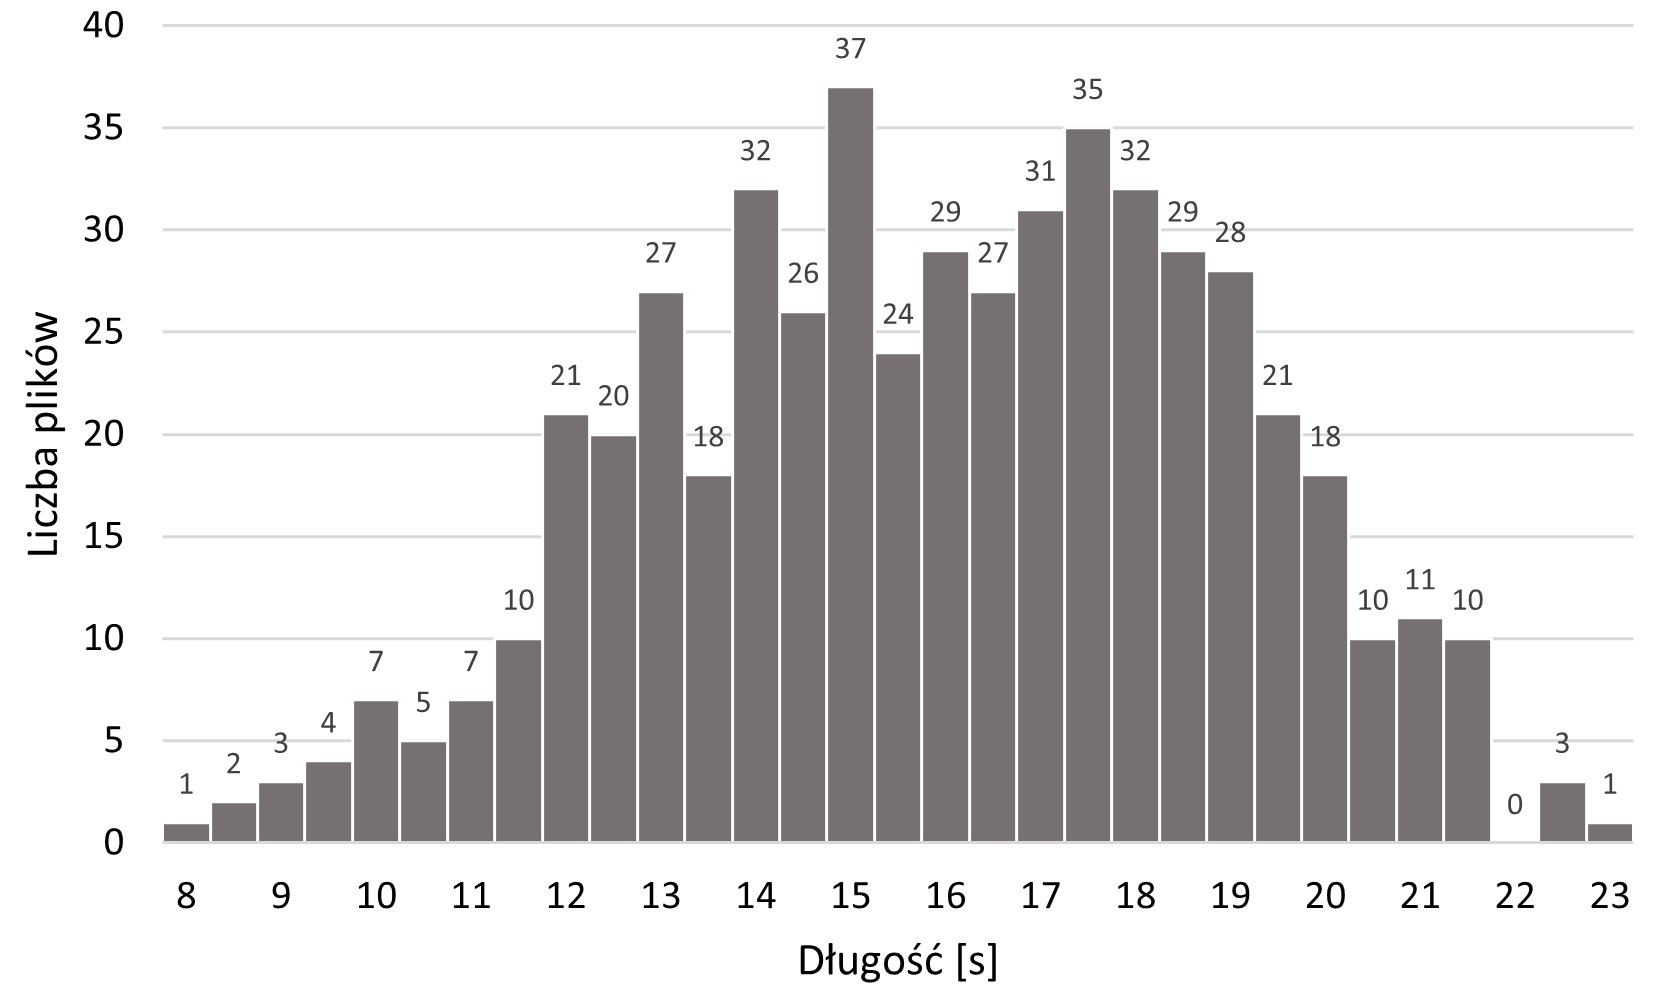
\includegraphics{img/histogram_gsd.jpg}
    \caption{Histogram długości nagrań w~bazie Speech Dataset.}
    \label{rysunek:histogram_gsd}
\end{figure}

\subsubsection*{Etykietowanie bazy}

Jak wyglądało etykietowanie bazy danych.
\section{Metoda}
\label{sec:metoda}

Opis tego jak zostało wykonane zadanie. Częściowo można odnosić się do tego z przeglądu literatury, ale nie powtarzać jeśli nie jest to absolutnie konieczne. Czytelnik w tym rozdziale ma się dowiedzieć JAK konkretnie zostało wykonane zadanie. Na podstawie tego rozdziału sam powinien móc w stanie powtórzyć badania.  

\subsection{Trening modelu}



\subsection{Ewaluacja modelu}

W metodzie zastosowano miarę zbalansowanej dokładności wyrażonej wzorem 
\begin{equation}
    \label{eqn:balanced_accuracy}
    ZD = \frac{(TP/(TP+FN))+(TN/(TN+FP))}{2},
\end{equation}
gdzie $TP$ oznacza wartości prawdziwe dodatnie, ...

\section{Wyniki}

To najważniejszy rozdział pracy, gdyż udowadnia co zostało zrobione. Powinien więc być tak napisany by opowiadał historię. Każde wyniki powinny być komentowane w kontekście celów pracy. Przykładowo całość retoryki można zbudować jako:

\subsection{Wyniki referencyjne}

Początkowo przeanalizowano system referencyjny składający się z (...). Tabela \ref{tab:wyniki1} przedstawia wyniki otrzymane dla pokoi o czasach pogłosów .... . Dane symulowane otrzymane metodą źródeł pozornych.

\begin{table}[h]
\centering
\caption{Skuteczność analizowanych metod wyrażona w mierze EER dla różnych czasów pogłosów.}
\begin{tabular}{@{}lllll@{}}
\toprule
Czas pogłosu RT60 {[}ms{]}      & 300          & 600          & 900          & 1200         \\ \midrule
Metoda 1                        & 3.5          & 4.5          & 4.9          & 7.3          \\
Algorytm 2                      & 2.5          & 3.3          & 3.9          & 6.8          \\
Zaproponowana metoda 2 & \textbf{1.5} & \textbf{2.7} & \textbf{3.0} & \textbf{4.5} \\ \bottomrule
\end{tabular}
\label{tab:wyniki1}
\end{table}

Wyniki w tabeli \ref{tab:wyniki1} wskazują, że metoda 2 jest lepsza niż metoda 1. Niemniej jednak zaproponowana w pracy metoda 3 umożliwia poprawę skuteczności ..... w warunkach pogłosowcyh.


Tu powinny znaleźć sie opisy otrzymanych wyników. Jeśli przeprowadzono kilka eksperymentów to warto tu opisać jak je osiągnięto. Wyniki powinno się raportować na wykresach, tabelach, histogramach, confussion matrix, scatter plot itp. 

\subsection{Porównanie}
Na koniec tego rozdziału jeśli wyników było sporo warto je podsumować 2-3 akapitami ogólnego komentarza, parafrazując część zdań z tego rozdziału.
\section{Podsumowanie}
% [MWI] Osiągnięto cele.

W podsumowaniu należy skomentować czy i jak udało sie zrealizować każdy cel pracy zdefiniowany w rozdziale \ref{subsec:cele_pracy}.Można posłużyć się podsekcjami jak niżej. 

% Pierwszym było opracowanie bazy nagrań mowy ze stresem, na które składało się nagranie możliwie największej liczby osób w~rzeczywistej sytuacji stresującej, odpowiednia unifikacja parametrów technicznych nagrań, opracowanie specyfikacji technicznej bazy, utworzenie narzędzia umożliwiającego etykietowanie zbioru nagrań oraz opracowanie i~analiza podstawowej wersji bazy zawierającej etykiety. Drugim celem była implementacja modułu detekcji stresu oraz ewaluacja jego skuteczności na zebranej bazie.

\subsubsection*{Cel 1}

Pierwszy cel został osiągnięty, poprzez sporządzenie bazy nagrań....

\subsubsection*{Implementacja modułu analizy ...}

Drugi cel zeralizowano implementując....

\subsubsection*{Optymalizacja metody}
Po implementacji metody usprawniono działanie poprzez ....

\addcontentsline{toc}{section}{Literatura}
\bibliography{bibliography.bib}
\bibliographystyle{plain}

\addcontentsline{toc}{section}{Załączniki}

\subsubsection*{Załącznik 1 - Kod umożliwiający etykietowanie bazy nagrań.}

Poniżej przedstawiono kod demonstrujący działanie narzędzia do etykietowania.

\definecolor{codegreen}{rgb}{0,0.6,0}
\definecolor{codegray}{rgb}{0.5,0.5,0.5}
\definecolor{codeorange}{rgb}{1,0.49,0}
\definecolor{backcolour}{rgb}{0.95,0.95,0.96}

\lstdefinestyle{mystyle}{
    backgroundcolor=\color{backcolour},
    commentstyle=\color{codegray},
    keywordstyle=\color{codeorange},
    numberstyle=\tiny\color{codegray},
    stringstyle=\color{codegreen},
    basicstyle=\fontsize{10}{10}\selectfont\ttfamily,
    breakatwhitespace=false,
    breaklines=true,
    captionpos=b,
    keepspaces=true,
    numbers=left,
    numbersep=5pt,
    showspaces=false,
    showstringspaces=false,
    showtabs=false,
    tabsize=2,
    xleftmargin=10pt,
}

\lstset{style=mystyle}

\begin{lstlisting}[language=Python, mathescape=true]
# import bibliotek
import os
from pathlib import Path
import random
import soundfile as sf
import sounddevice as sd


with open("labels.txt", "a") as f:
    for idx, filestem in enumerate(files):
        # zapisanie numeru opisywanego pliku 
        # do zmiennej "file_number"
        file_number = int(len(done_files)) + int(idx) + 1
        while True:
            # zapisanie sciezki do opisywanego pliku 
            # do zmiennej "filename"
            filename = (
                f"speech_dataset/{str(filestem)}.flac"
            )

          

\end{lstlisting}
\end{document}

